\documentclass[onecolumn,10pt]{article}
 \textheight = 23.4cm
 \textwidth = 18cm
 \topmargin = -2cm
 \oddsidemargin= -1cm
 \parindent = 0mm
\usepackage[english]{babel}
\usepackage{graphicx}
\graphicspath{ {/home/Dropbox/Digital2/Laboratorio/Lab1} }
%\selectlanguage{spanish}
%\usepackage[spanish]{babel}
\usepackage[latin1]{inputenc}
\usepackage{times}
\usepackage{amssymb,amsfonts}
\usepackage[tbtags]{amsmath}
\usepackage{cite}
\usepackage{float}
\setlength{\columnsep}{7mm}

%-----------------------------------------------------------------------

%-----------------------------------------------------------------------
\begin{document}
\title{Proyecto Final: Secador de Cafe}
\author{Albin Gonzalo Rodriguez\\Diego Fernando Chaparro\\ Elkin Alejandro Romero \\
Electronica Digital II\\ Docente: Diego Alexander Tibaduiza\\ Universidad Nacional de Colombia - Sede Bogota\\
Departamento de Ingenier�a El�ctrica, Electr�nica y Computaci�n\\}
\maketitle



\begin{abstract}
In this project we will present a solution to our problem of drying the coffee to optimize the production. It consists of a system of monitoring and control of environment inside a dryer. Therefore we will control variables of temperature and humidity so that the drying time is shorter and so we can automate drying.
\end{abstract}


\section{Palabras claves}

Secador, sensores de temperatura y humedad, modulo wifi, display.


\section{Introducci�n}

En este proyecto vamos a presentar una solucion a nuestro problema de secado del cafe para asi optimizar la producci�n. Consiste en un sistema de monitoreo y control de ambiente dentro de un secador. Por lo tanto vamos a controlar variables de temperatura y humedad para que el tiempo de secado sea menor y asi poder automatizar el secado. 

\section{Marco teorico}

\subsection{Problema}

Encontramos que en el secador hay variaciones de temperatura y humedad por el clima, por lo tanto nos produce un da�o a las caracteristicas del cafe. 

Ahora el tiempo de secado es mucho mayor que en un sistema controlado y monitoreado. Eso nos permite modelar y automatizar un sistema, para que el secado del cafe sea mucho menor. 

En la siguiente figura vamos a mostrar como se comportan las variables de temperatura y humedad, en el cual esta actualmente el secador.

\begin{figure}[H]
  % Requires \usepackage{graphicx}
 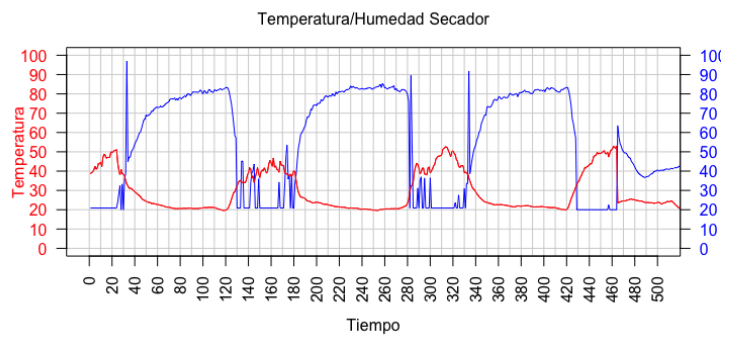
\includegraphics[width=18cm,height=4.5cm]{Ima9.png}\\
  %\caption{Variables de Temperatura y Humedad}\label{fig:1}
\end{figure}

\subsection{Requerimientos}
Se quiere monitorear y controlar temperatura y humedad en una edificaci�n para el secado de caf� (secador) con un volumen aproximado de $180 m^3$, donde el caf� se almacena en estanter�as perforadas para permitir el flujo de aire de 3 niveles. Las variables a monitorear/controlar son temperatura (no mayores a 38 grados celsius) y una humedad (inferior a 40\%) para obtener un secado optimo y as� reducir el tiempo de secado. La toma de medidas de los sensores se realizar� cada 5 minutos con dos parejas de sensores humedad/temperatura ubicados, uno en dentro del secador y el otro en la parte exterior, cuando el valor promedio se aproxime de forma ascendente a 38 grados se accionan dos extractores ubicados en los extremos. Se quiere que la informaci�n generada por los sensores sobre el secador est� disponible para consulta en un servidor ubicado en la finca y que la informaci�n se almacene en el servidor cuando este se encienda, cada dato se almacena en una memoria flash sh en intervalos de tiempo de 5 minutos, Mientras no exista un lote de cafe en el secador el sistema no deber� funcionar.



\subsection{Antecedentes}

\begin{figure}[H]
  % Requires \usepackage{graphicx}
 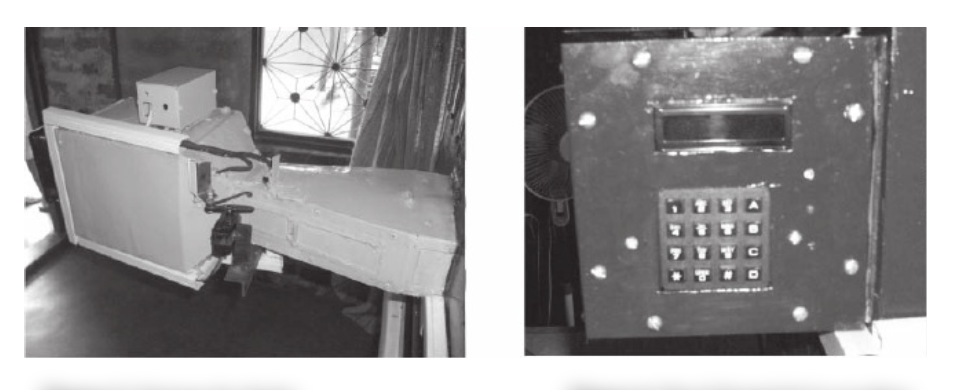
\includegraphics[width=18.5cm,height=5.5cm]{Ima1.png}\\
  \caption{Antecedentes}\label{fig:2}
\end{figure}
\begin{figure}[H]
  % Requires \usepackage{graphicx}
 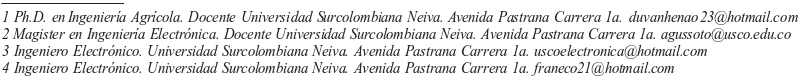
\includegraphics[width=18.5cm,height=2cm]{Ima2.png}\\
  \caption{Autores}\label{fig:3}
\end{figure}
\begin{figure}[H]
  % Requires \usepackage{graphicx}
 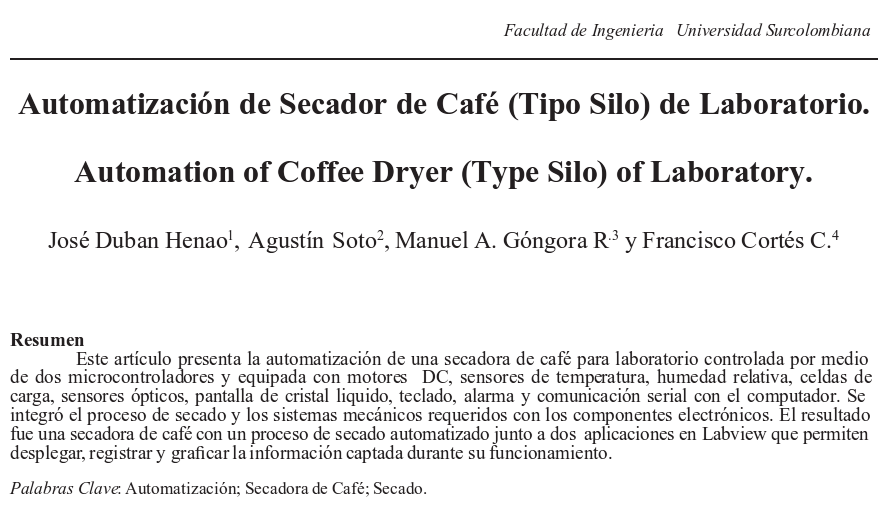
\includegraphics[width=18.5cm,height=10cm]{Ima3.png}\\
  %\caption{Documento}\label{fig:3}
\end{figure}


\subsection{PESTEL}

\begin{figure}[H]
  % Requires \usepackage{graphicx}
 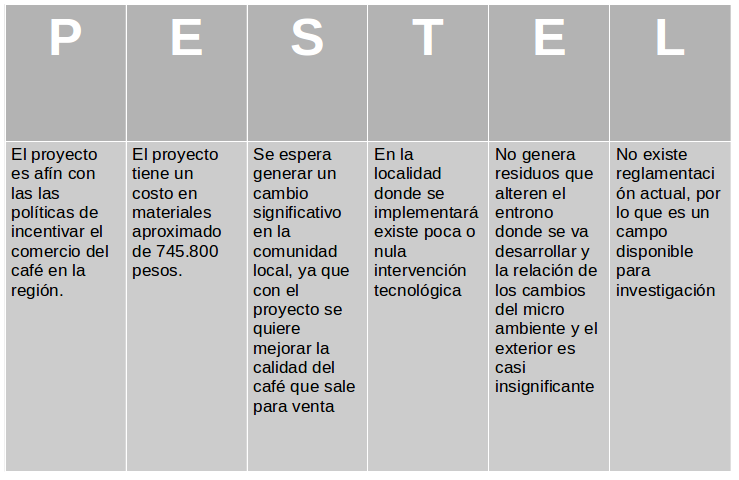
\includegraphics[width=18.5cm,height=10cm]{Ima4.png}\\
  \caption{Tabla de PESTEL}\label{fig:4}
\end{figure}


\subsection{Actores}


\begin{figure}[H]
  % Requires \usepackage{graphicx}
 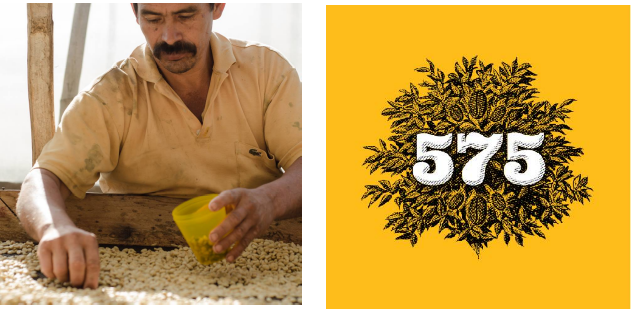
\includegraphics[width=18.5cm,height=7cm]{Ima5.png}\\
  \caption{Actores}\label{fig:5}
\end{figure}

En nuestro caso los actores son: El secado del cafe y la empresa donde nos va a financiar el proyecto. Asi como lo muestra la figura \ref{fig:5}. 


\subsubsection{Secador}

\begin{figure}[H]
  % Requires \usepackage{graphicx}
 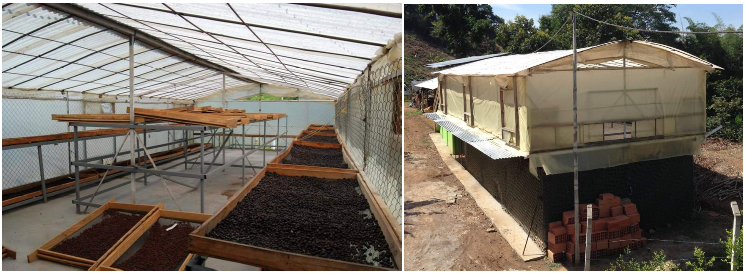
\includegraphics[width=18.5cm,height=7cm]{Ima6.png}\\
  \caption{Secador}\label{fig:6}
\end{figure}

En la figura \ref{fig:5} podemos evidenciar que hay varias variables que afectan el secador directamente, como lo son: El suelo, la temperatura de ambiente, la temperatura del secador, el ambiente, la humedad entre otros.


\subsection{Propuesta}
Nuestra propuesta es hacer un secado en menor tiempo. Para eso necesitamos de sensores(Para obtener informaci�n del ambiente en un lapso de tiempo), memoria sd (Para guardar los datos obtenidos de cada sensor), display(Para poder mostrar la informacion de los sensores) y un modulo wifi, para que actuen en el momento que se requiera un cambio de temperatura o humedad. 

\begin{figure}[H]
  % Requires \usepackage{graphicx}
 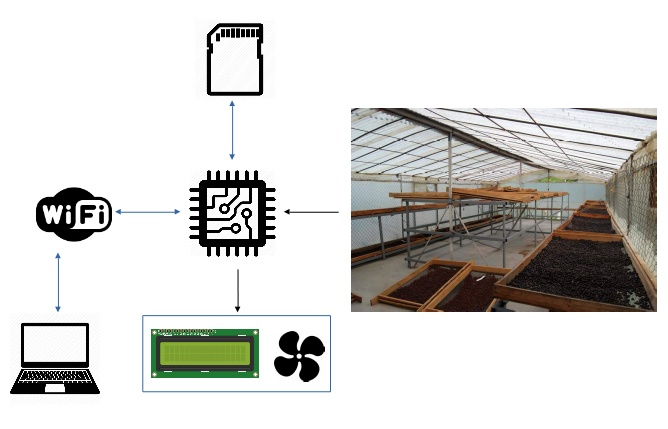
\includegraphics[width=18.5cm,height=7cm]{Ima7.png}\\
  \caption{Propuesta}\label{fig:7}
\end{figure}



\subsection{Objetivos}
\begin{itemize}
\item Ya planteada una solucion del problema, vamos a realizar diferentes posibilidades de desarrollo, para que la optimizacion de la produccion del caf� sea mejor.

\item Controlar el secador por medio de microprosesadores, sensores de humedad, sensores de temperatura, modulos wifi, pantallas lcd y almacenamiento en sd.

\item Opimizar costos por medio de la automatizacion. 
\end{itemize}

\subsection{Costos}

\begin{figure}[H]
  % Requires \usepackage{graphicx}
 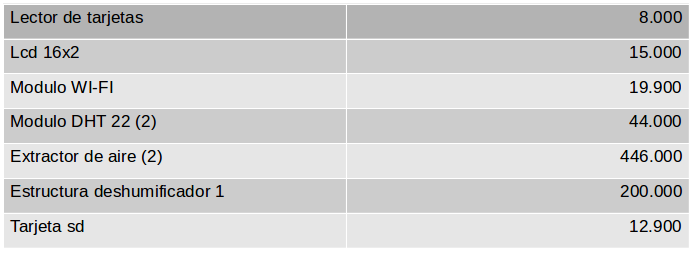
\includegraphics[width=18.5cm,height=5cm]{Ima8.png}\\
  \caption{Costo total: 745.800}\label{fig:8}
\end{figure}

%\begin{equation*}
 %   V=R*I
%\end{equation*}


\section{Procedimiento}
En el proyecto hemos avanzado en la inclusi�n de varios modulos, los cuales son: SPI-flash-controll al procesador LM32, Pantalla LCD - I2C y modulo Wifi.

Para ver los avances del proyecto vamos a tomar unas fotos de que se ha hecho y los problemas que hemos tenido para terminar el proyecto.
\subsection{Wiki}

\begin{figure}[H]
  % Requires \usepackage{graphicx}
 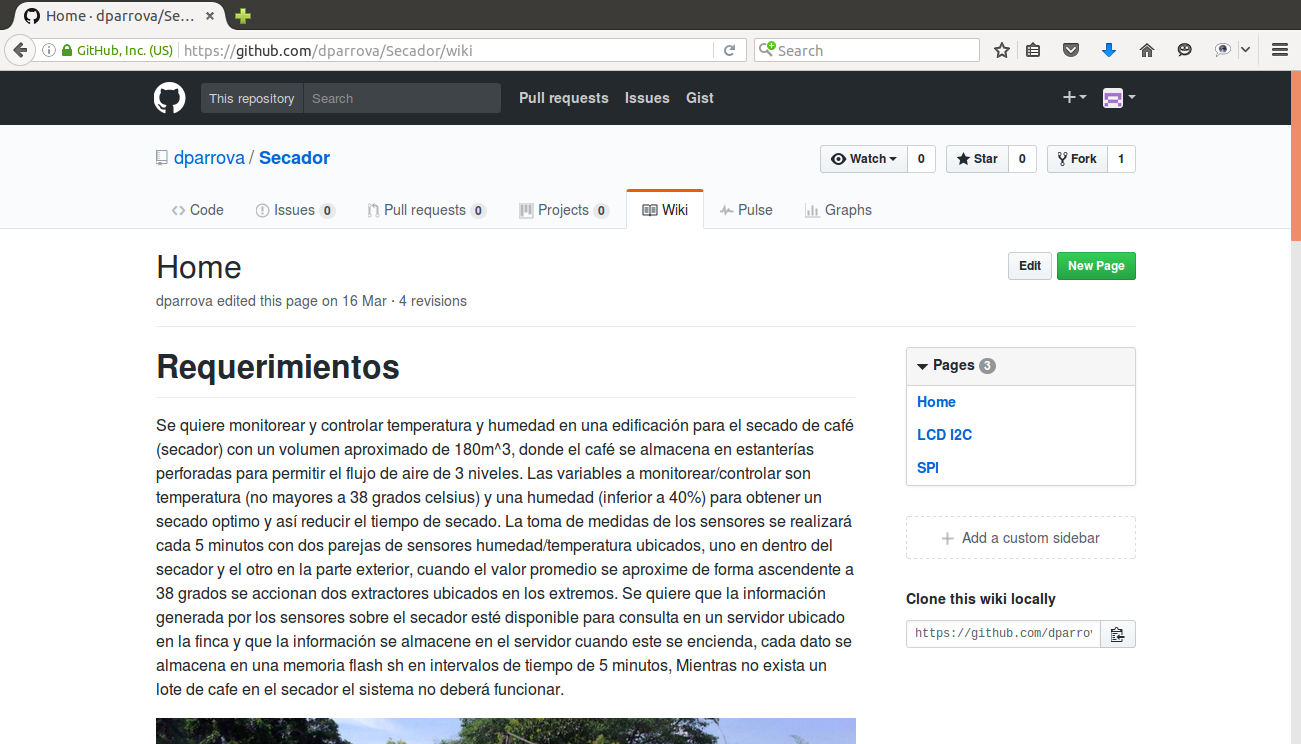
\includegraphics[width=18.5cm,height=12cm]{Ima10.png}\\
  \caption{Wiki}\label{fig:9}
\end{figure}

\subsection{Codigo}

\begin{figure}[H]
  % Requires \usepackage{graphicx}
 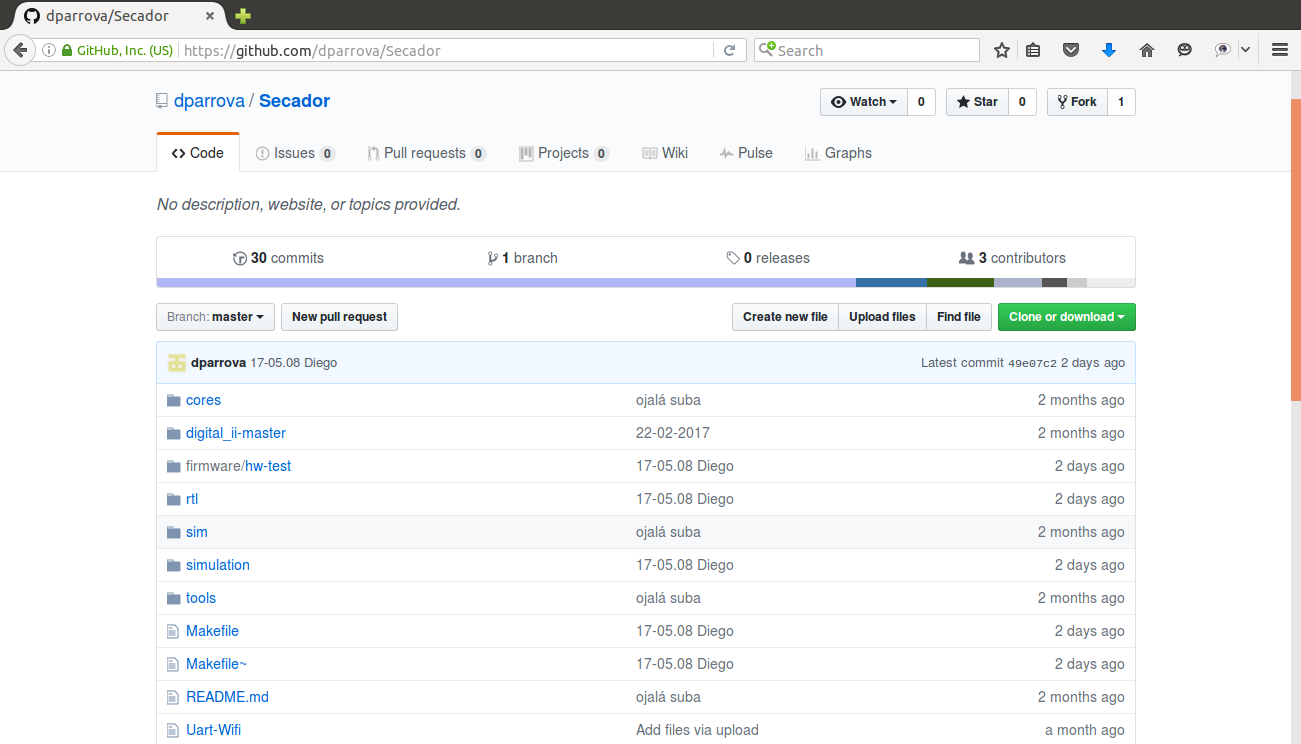
\includegraphics[width=18.5cm,height=9cm]{Ima11.png}\\
  \caption{Codigo 1}\label{fig:10}
\end{figure}
\begin{figure}[H]
  % Requires \usepackage{graphicx}
 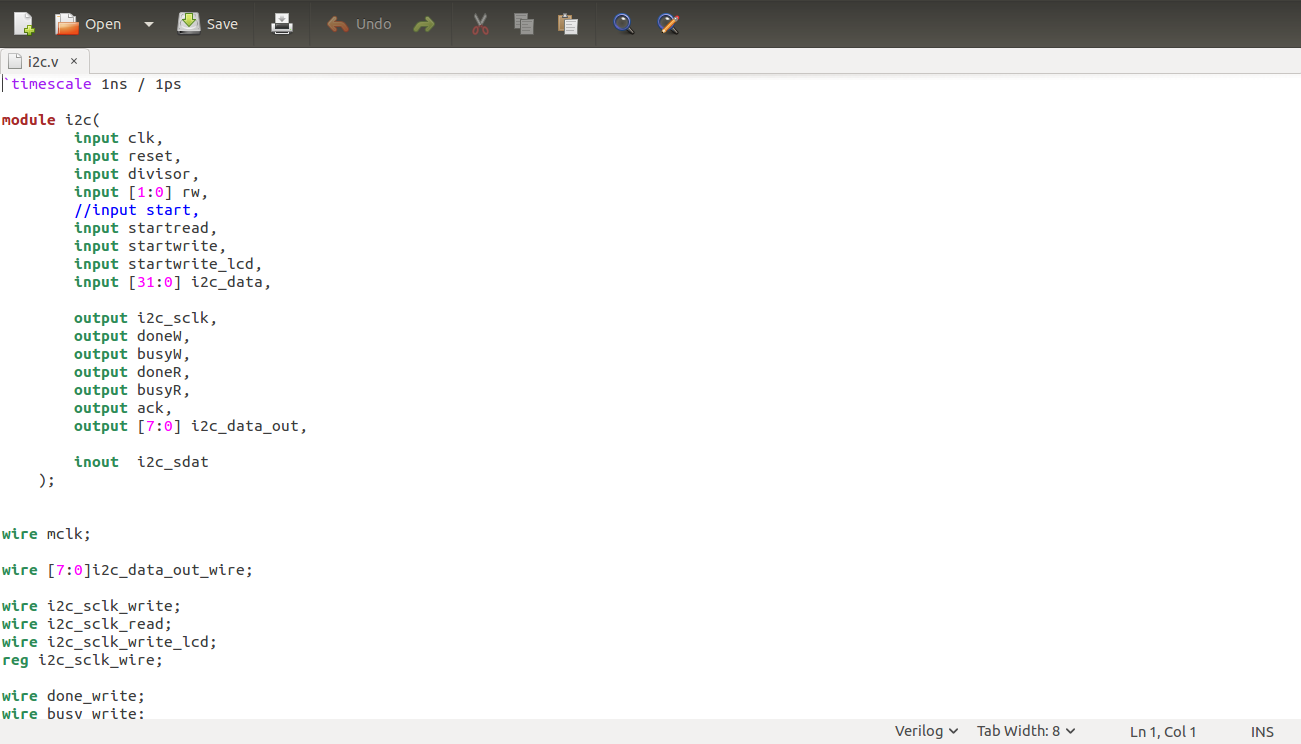
\includegraphics[width=18.5cm,height=9cm]{Ima12.png}\\
  \caption{Codigo 2}\label{fig:11}
\end{figure}

\subsection{Simulaciones}

\begin{figure}[H]
  % Requires \usepackage{graphicx}
 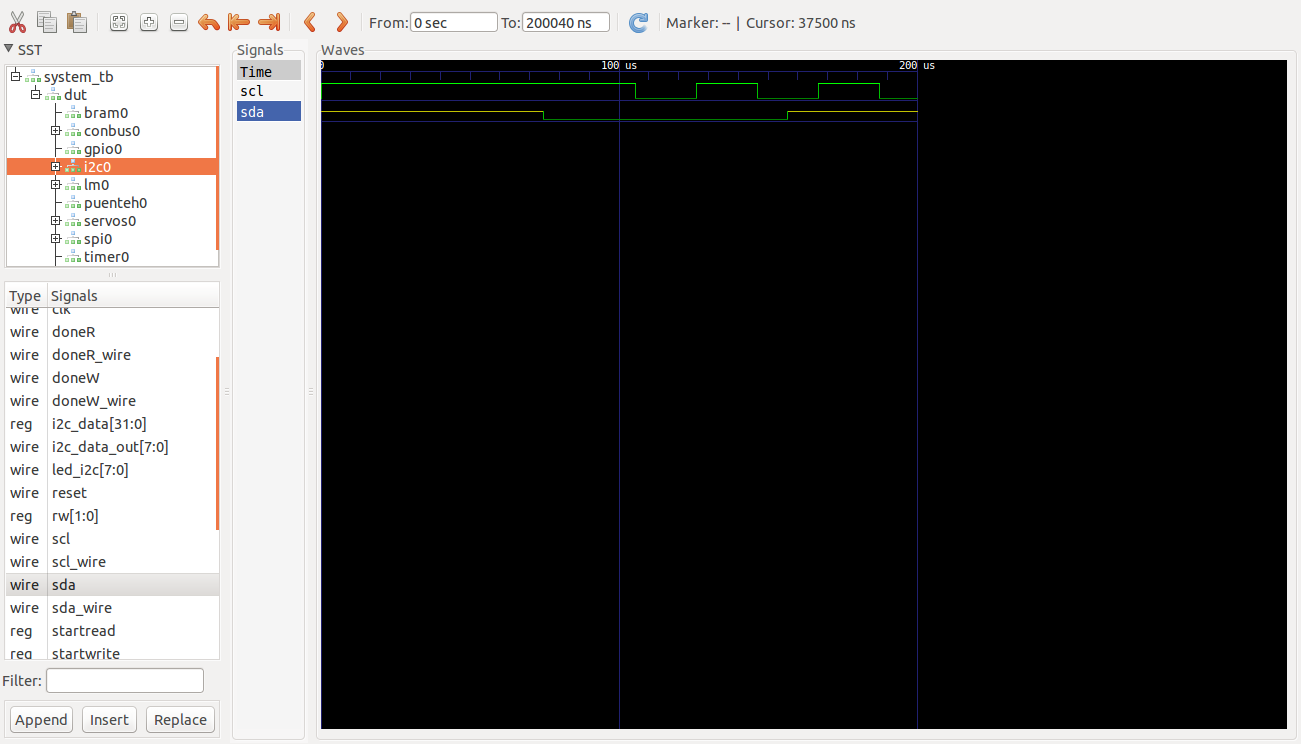
\includegraphics[width=18.5cm,height=12cm]{Ima13.png}\\
  \caption{Simulacion I2C-LCD}\label{fig:12}
\end{figure}

\subsection{Proyecto Fisico}

\begin{figure}[H]
  % Requires \usepackage{graphicx}
 \begin{center}
 
 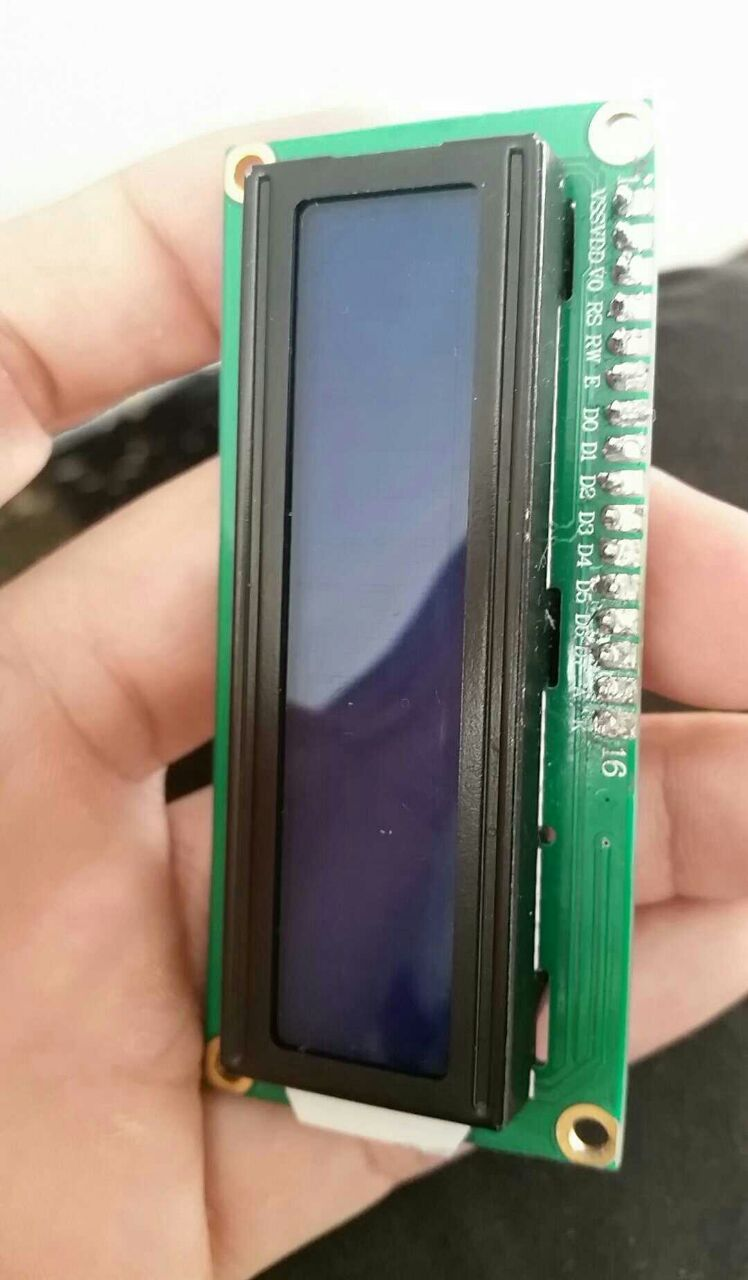
\includegraphics[width=8.5cm,height=3cm]{Ima14.jpg}\\
  \caption{Panta LCD}\label{fig:13}

 \end{center}
\end{figure}
\begin{figure}[H]
  % Requires \usepackage{graphicx}
 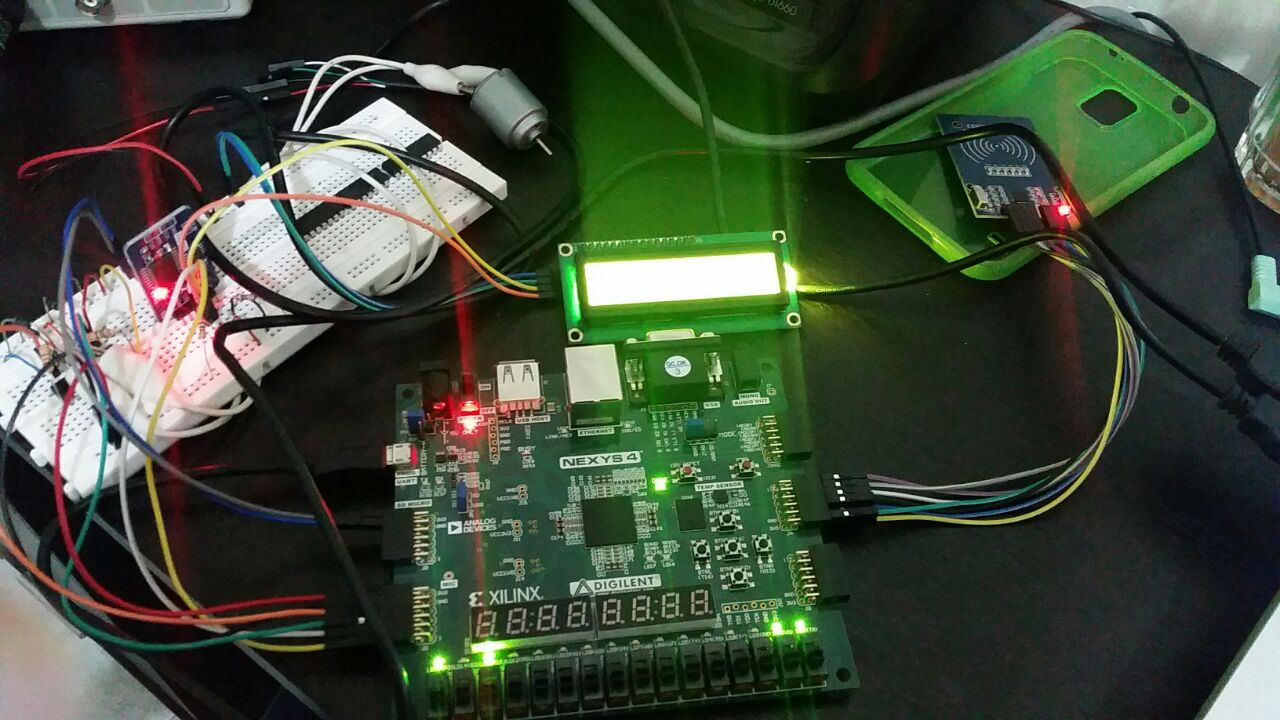
\includegraphics[width=18.5cm,height=9cm]{Ima15.jpg}\\
  \caption{Proyecto fisico: LCD}\label{fig:14}
\end{figure}
\begin{figure}[H]
  % Requires \usepackage{graphicx}
 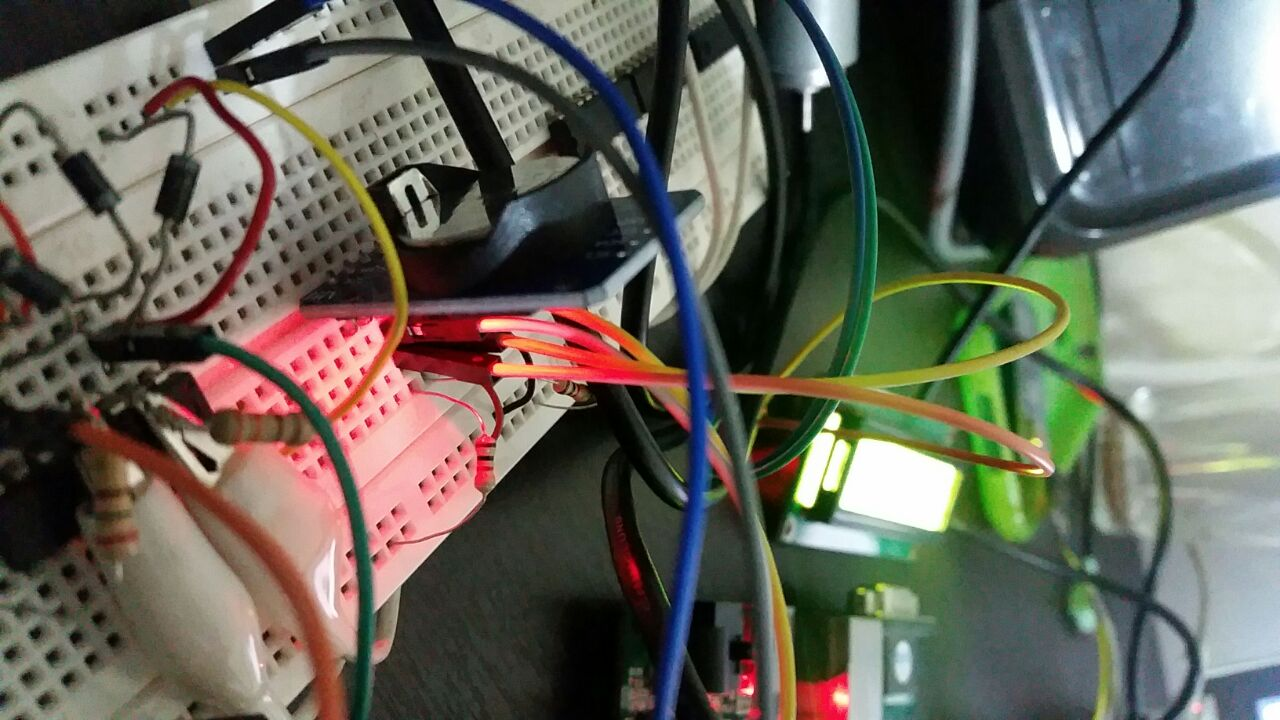
\includegraphics[width=18.5cm,height=9cm]{Ima16.jpg}\\
  \caption{Modulo Wifi}\label{fig:15}
\end{figure}

\subsection{Problemas}
\begin{itemize}
\item Hemos tenido problemas con la sincronizacion del reloj en algunos modulos
\item Tambien se han presentado problemas en la conexion de todos los modulos juntos, puesto que la memoria no alcanza para varios modulos por lo tanto necesitamos otra fpga o otro dispositivo.
\item Hemos tenido problemas en algunos codigos descargados.
\end{itemize}



\section{Conclusiones}
\begin{itemize}
  \item En conclusion nosotros podemos controlar por medio de la automatizacion y la arquitectura de computadores, diferentes medios como lo puede ser un clima en un citio cerrado 
  \item Tambien podemos apreciar que la conexion de los modulos con el procesador es importante para que el proyecto funcione de manera optima 
  \item En cuanto a los problemas que hemos evidenciado, trataremos de solucionarlos en el menor tiempo posible
\end{itemize}

\section{Bibliografia}

\begin{itemize}
  \item Wiki: https://github.com/algrodriguezrol/Secador
  \item https://github.com/dparrova/Secador/wiki
  \item https://www.scribd.com/doc/157353212/AUTOMATIZACION-DE-SECADOR-DE-CAFE-TIPO-SILO-DE-LABORATORIO
   \item http://github.com/dparrova/secador
\item www.freeiconspng.com
\item https://www.iconfinder.com
\item http://www.coffeeresearch.org/agriculture/drying.htm
\item http://www.latticesemi.com/en/Products/DesignSoftwareAndIP/IntellectualProperty/ReferenceDesigns/ReferenceDesigns01/SPIFlashControllerwithWearLeveling.aspx
 
\item https://www.facebook.com/575cafe/
\end{itemize}

\end{document}
